\subsection{Системы небесных координат}
Каждая из систем небесных координат является сферической системой координат, в которой радиус не имеет значения, так как параллакс не учитывается, а объекты считаются бесконечно удалёнными от наблюдателя.

\begin{figure}[!h]
	\centering
	\begin{subcaptionblock}{0.49\textwidth}
		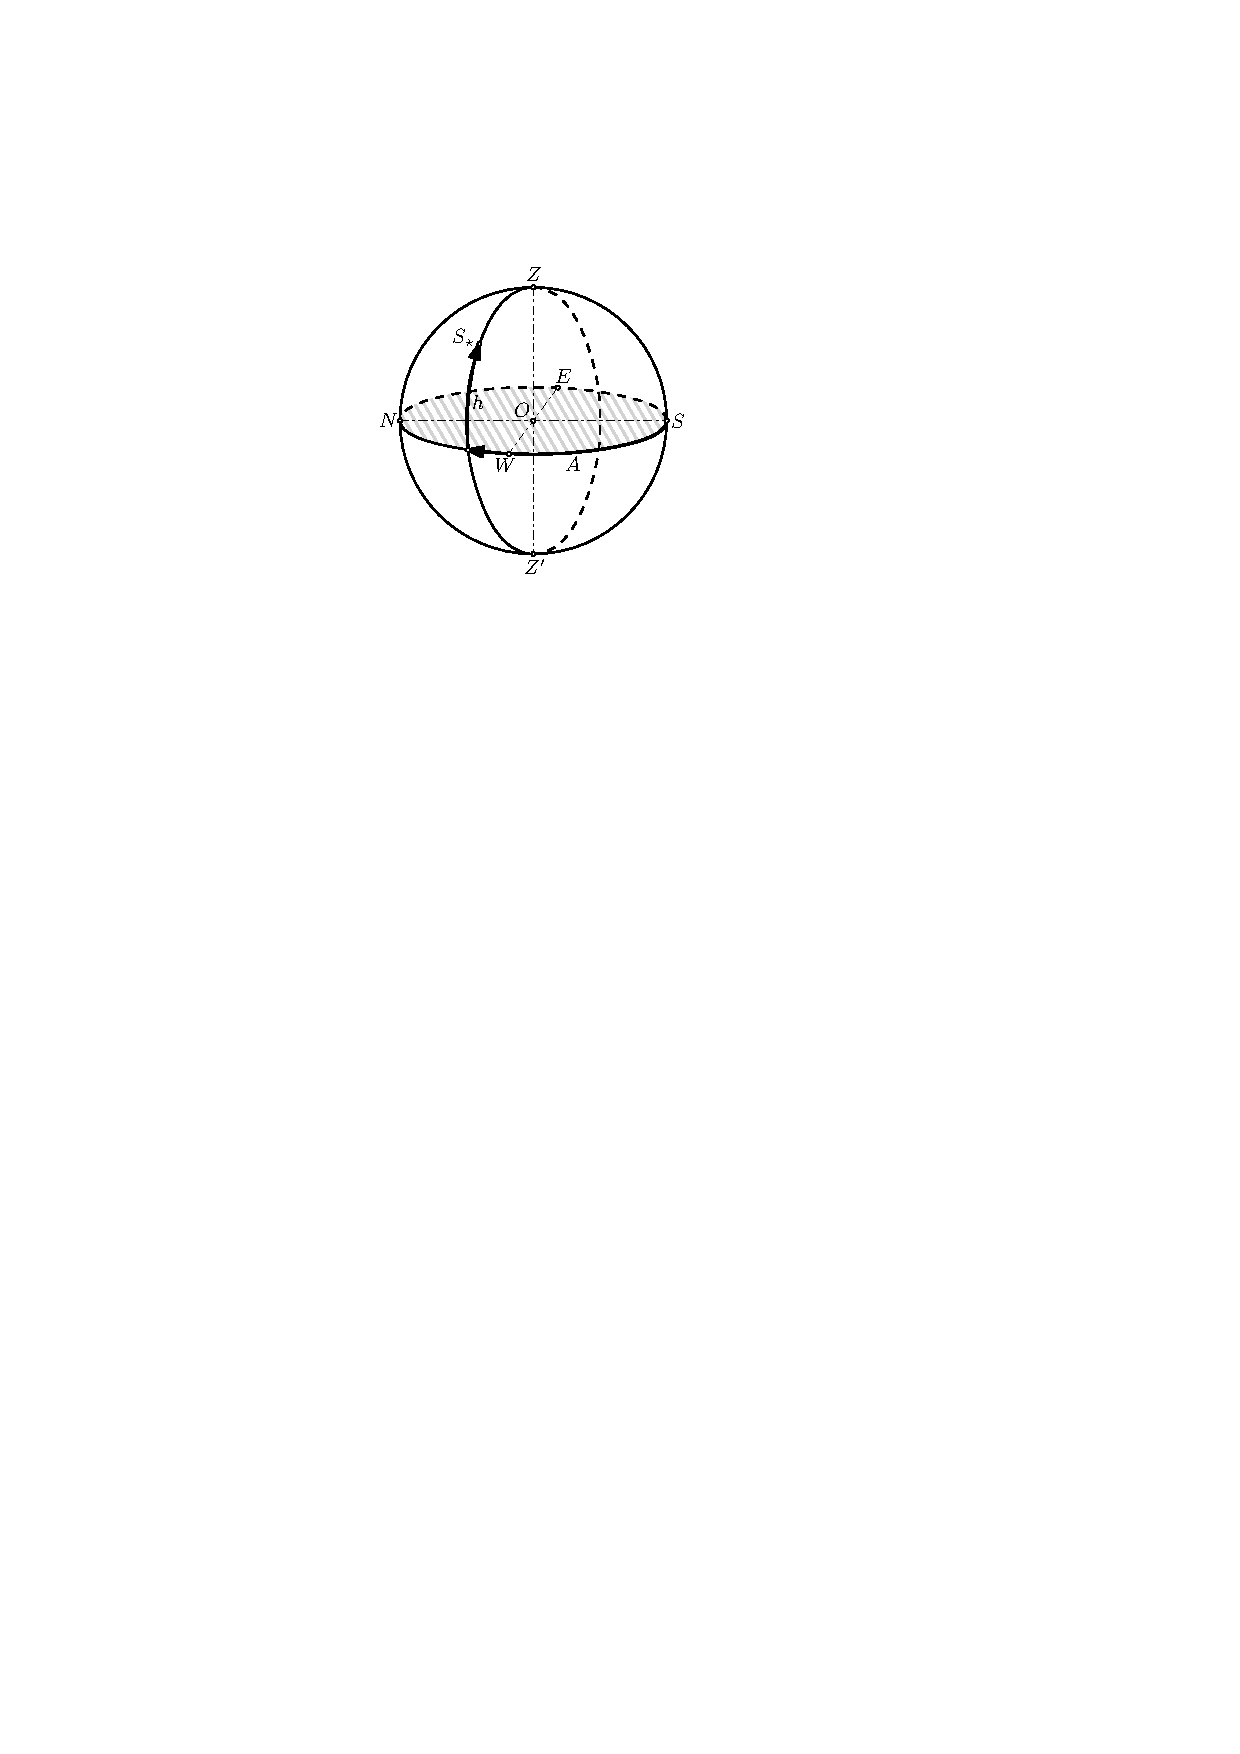
\includegraphics[width = \textwidth]{hor-coordin-sys}
		\caption{Горизонтальная система координат}
	\end{subcaptionblock}
	\hfill
	\begin{subcaptionblock}{0.49\textwidth}
		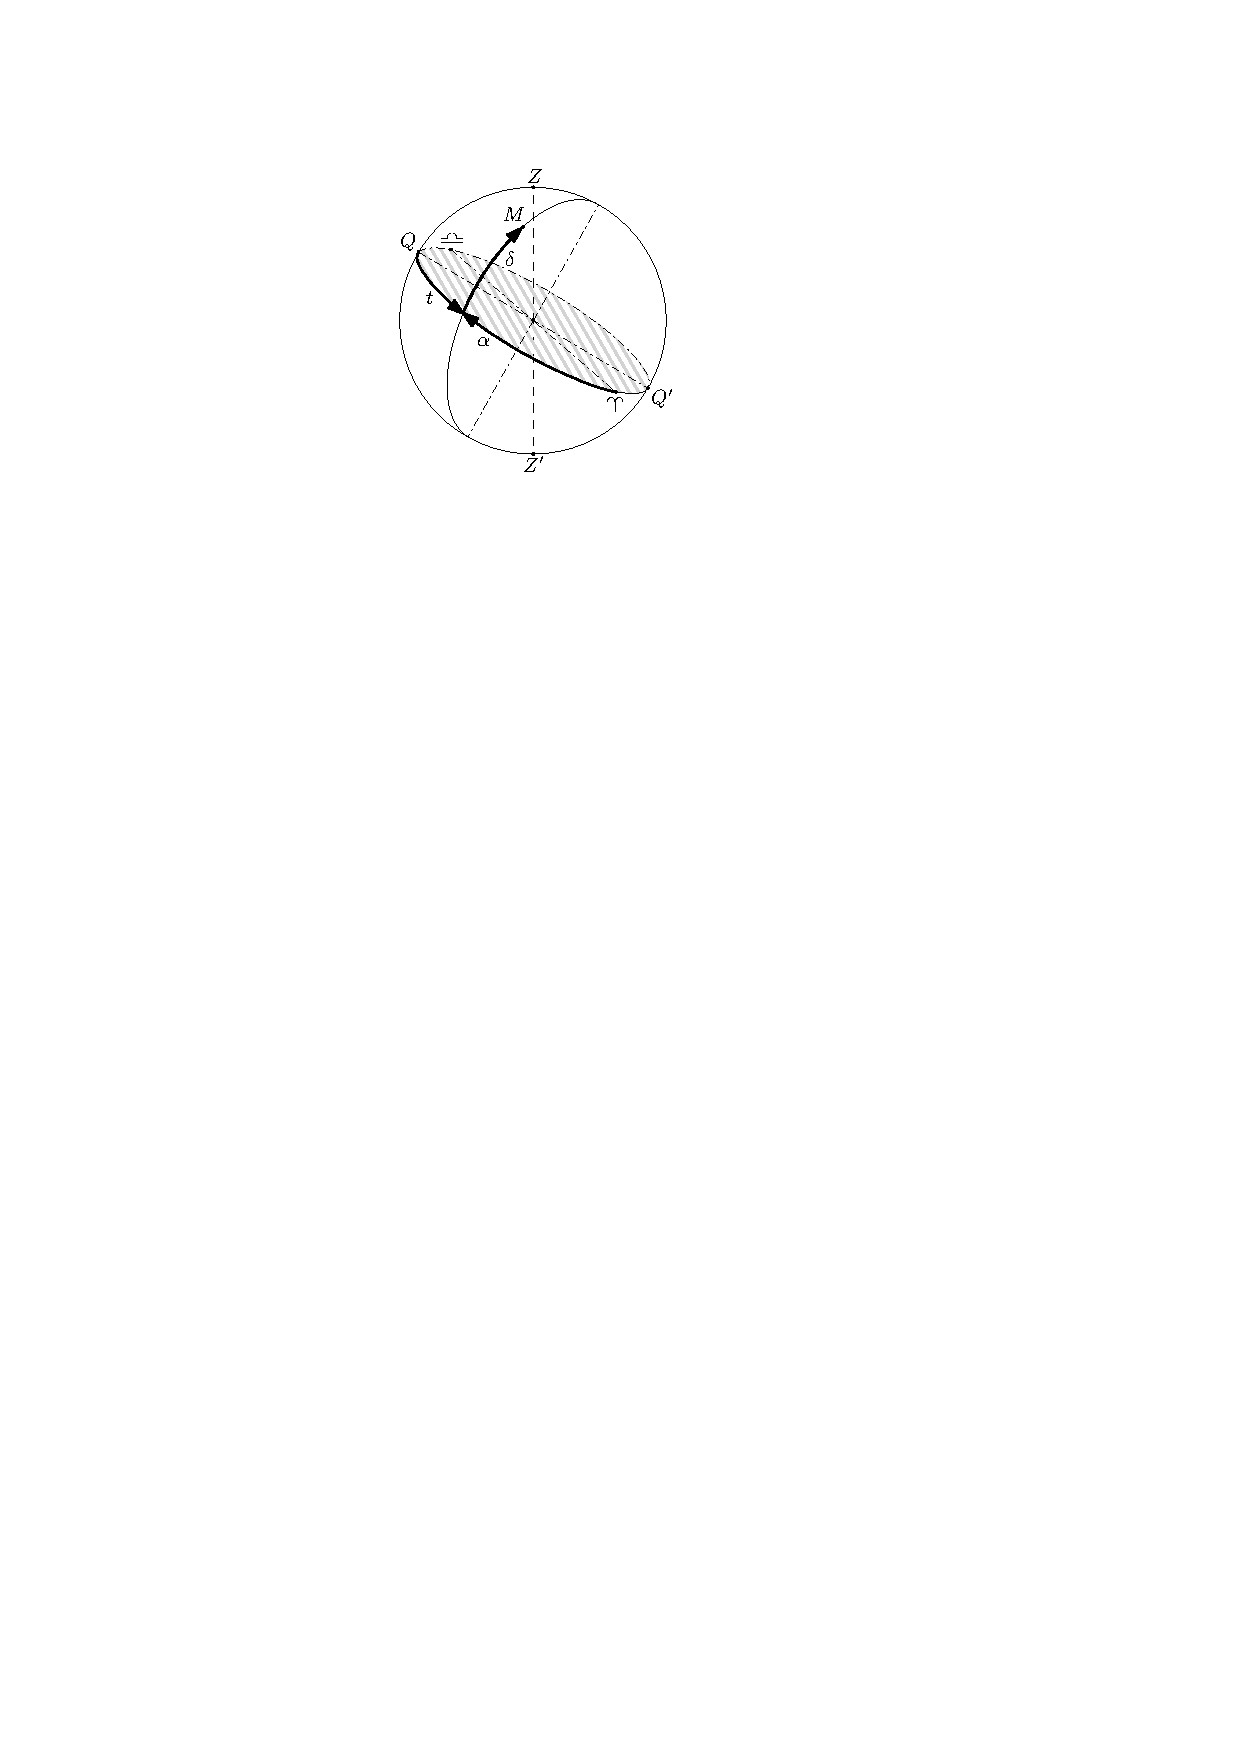
\includegraphics[width = \textwidth]{eq-coordin-sys}
		\caption{Экваториальная система координат}
	\end{subcaptionblock}
	\caption{Системы координат I}
\end{figure}
\term{Горизонтальная система координат}~--- система координат, в которой основной плоскостью является плоскость математического горизонта, а полюсами~--- \term{зенит} и \term{надир}~--- точки небесной сферы, расположенные ровно над наблюдателем и под ним соответственно. Одной координатой является либо \term{высота} светила $h$~--- угловое расстояние между светилом и математическим горизонтом, отсчитываемое в сторону зенита, либо его \term{зенитное расстояние}~$z$~--- угловое расстояние между зенитом и светилом. Другой координатой является \term{астрономический азимут} $A$~--- угол $SZS_\star$, отсчитываемый в сторону запада. Половина большого круга, перпендикулярного горизонту,~--- $Z S_\star Z'$  называется \term{вертикалом} объекта.

\term[экваториальная система координат]{Первая экваториальная система координат}~--- система координат,
основной плоскостью которой является плоскость небесного экватора $QEQW'$.
Одной координатой при этом является \term{склонение}~$\delta$~--- угловое
расстояние между светилом и плоскостью небесного экватора, отсчитываемое в
сторону севера. Половина большого круга, вдоль которой отсчитывается склонение,
перпендикулярна небесному экватору и называется \term[круг склонений]{кругом склонений} или
\imp{кругом равных часовых углов (прямых восхождений)}. Наряду со склонением
используется \term{полярное расстояние}~$p$~--- угловое расстояние между
светилом и полюсом мира. Другой координатой является \term{часовой угол}~$t$~---
дуга небесного экватора от верхней точки небесного экватора до круга склонения
светила в сторону запада, или угол между небесным меридианом и кругом склонения
светила. $\aries$ и $\libra$~--- точки весеннего и осеннего равноденствия соответственно.

\term[экваториальная система координат]{Вторая экваториальная система координат}~--- система, аналогичная предыдущей. Одной координатой по прежнему является \term{склонение}~$\delta$. А другой координатой является \term{прямое восхождение}~$\alpha$~--- угловое расстояние между точкой весеннего равноденствия и кругом склонений светила в сторону годичного движения Солнца.

\begin{figure}[!h]
	\centering
	\begin{subcaptionblock}{0.49\textwidth}
		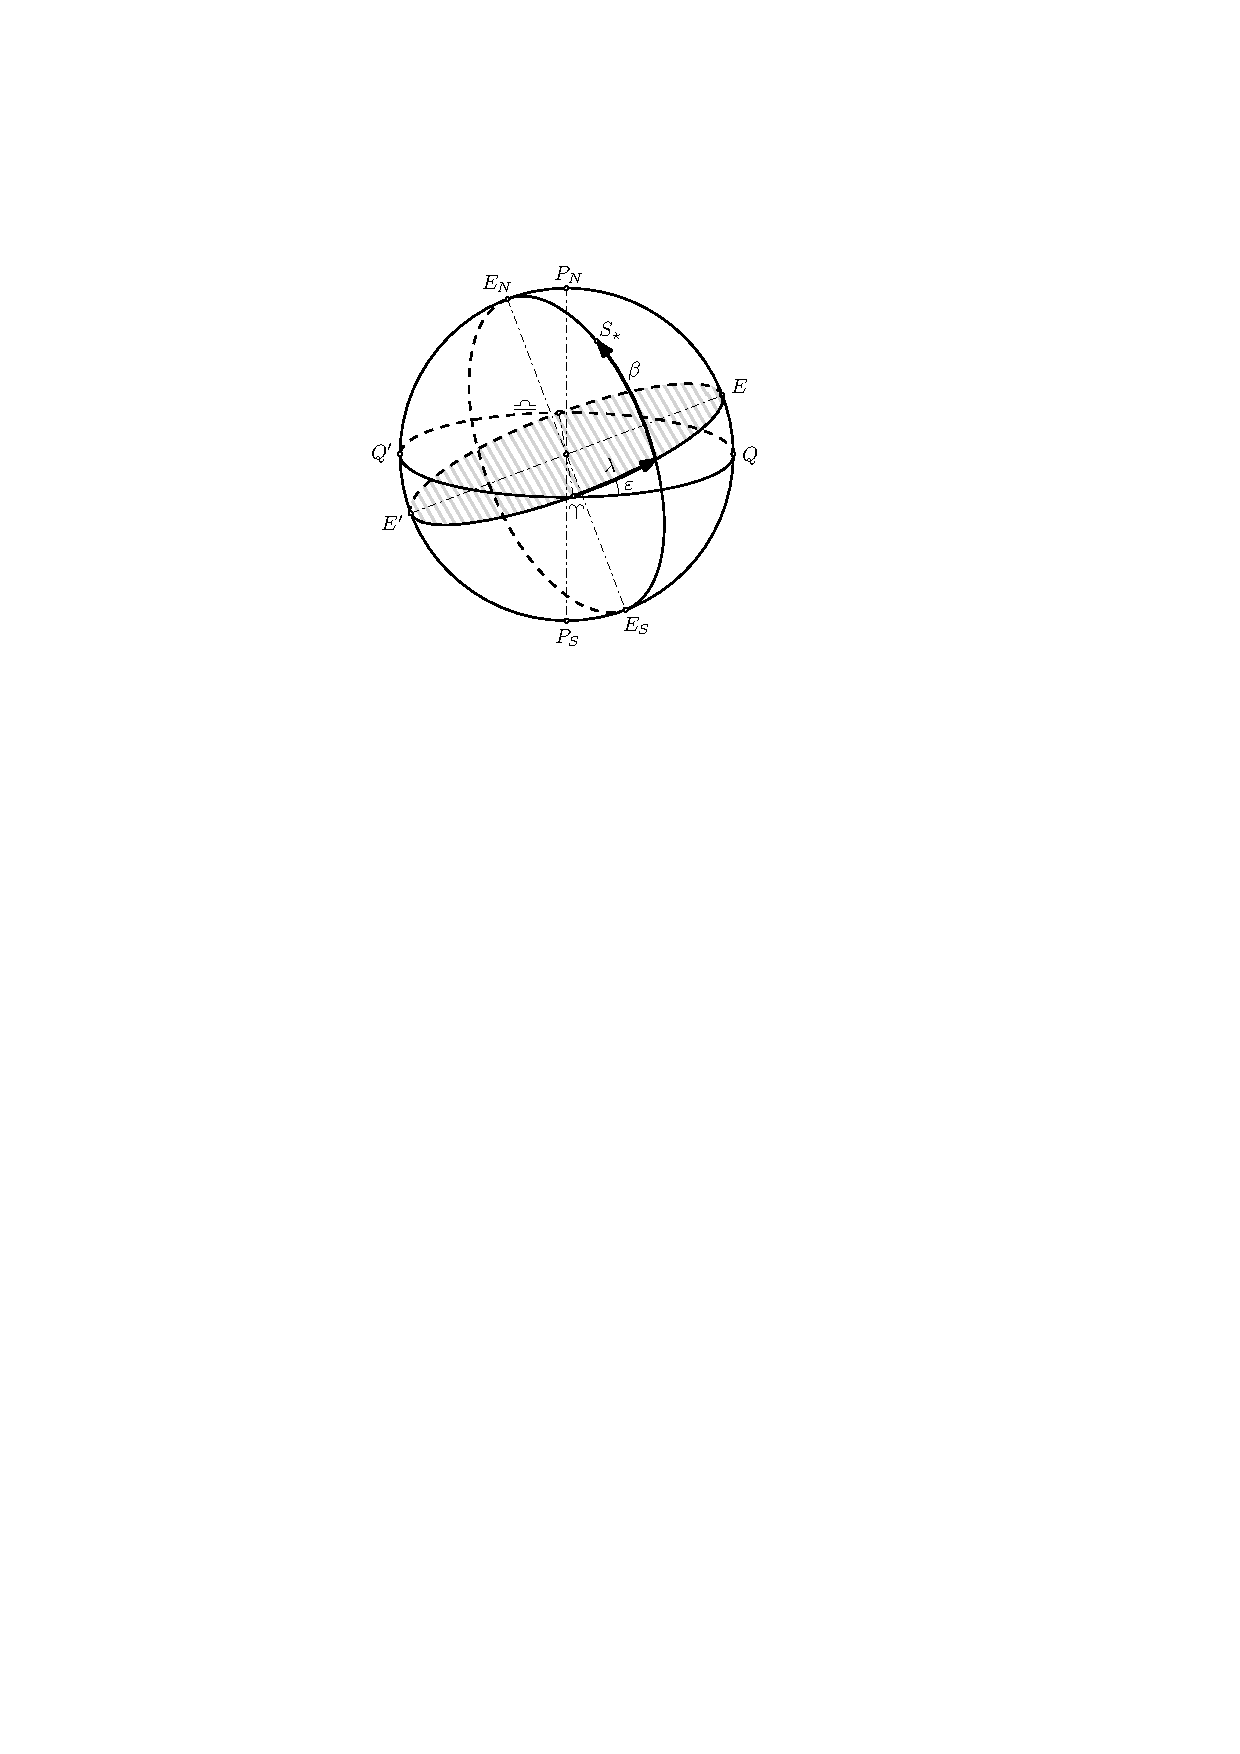
\includegraphics[width = \textwidth]{eql-coordin-sys}
		\caption{Эклиптическая система координат}
	\end{subcaptionblock}
	\hfill
	\begin{subcaptionblock}{0.49\textwidth}
		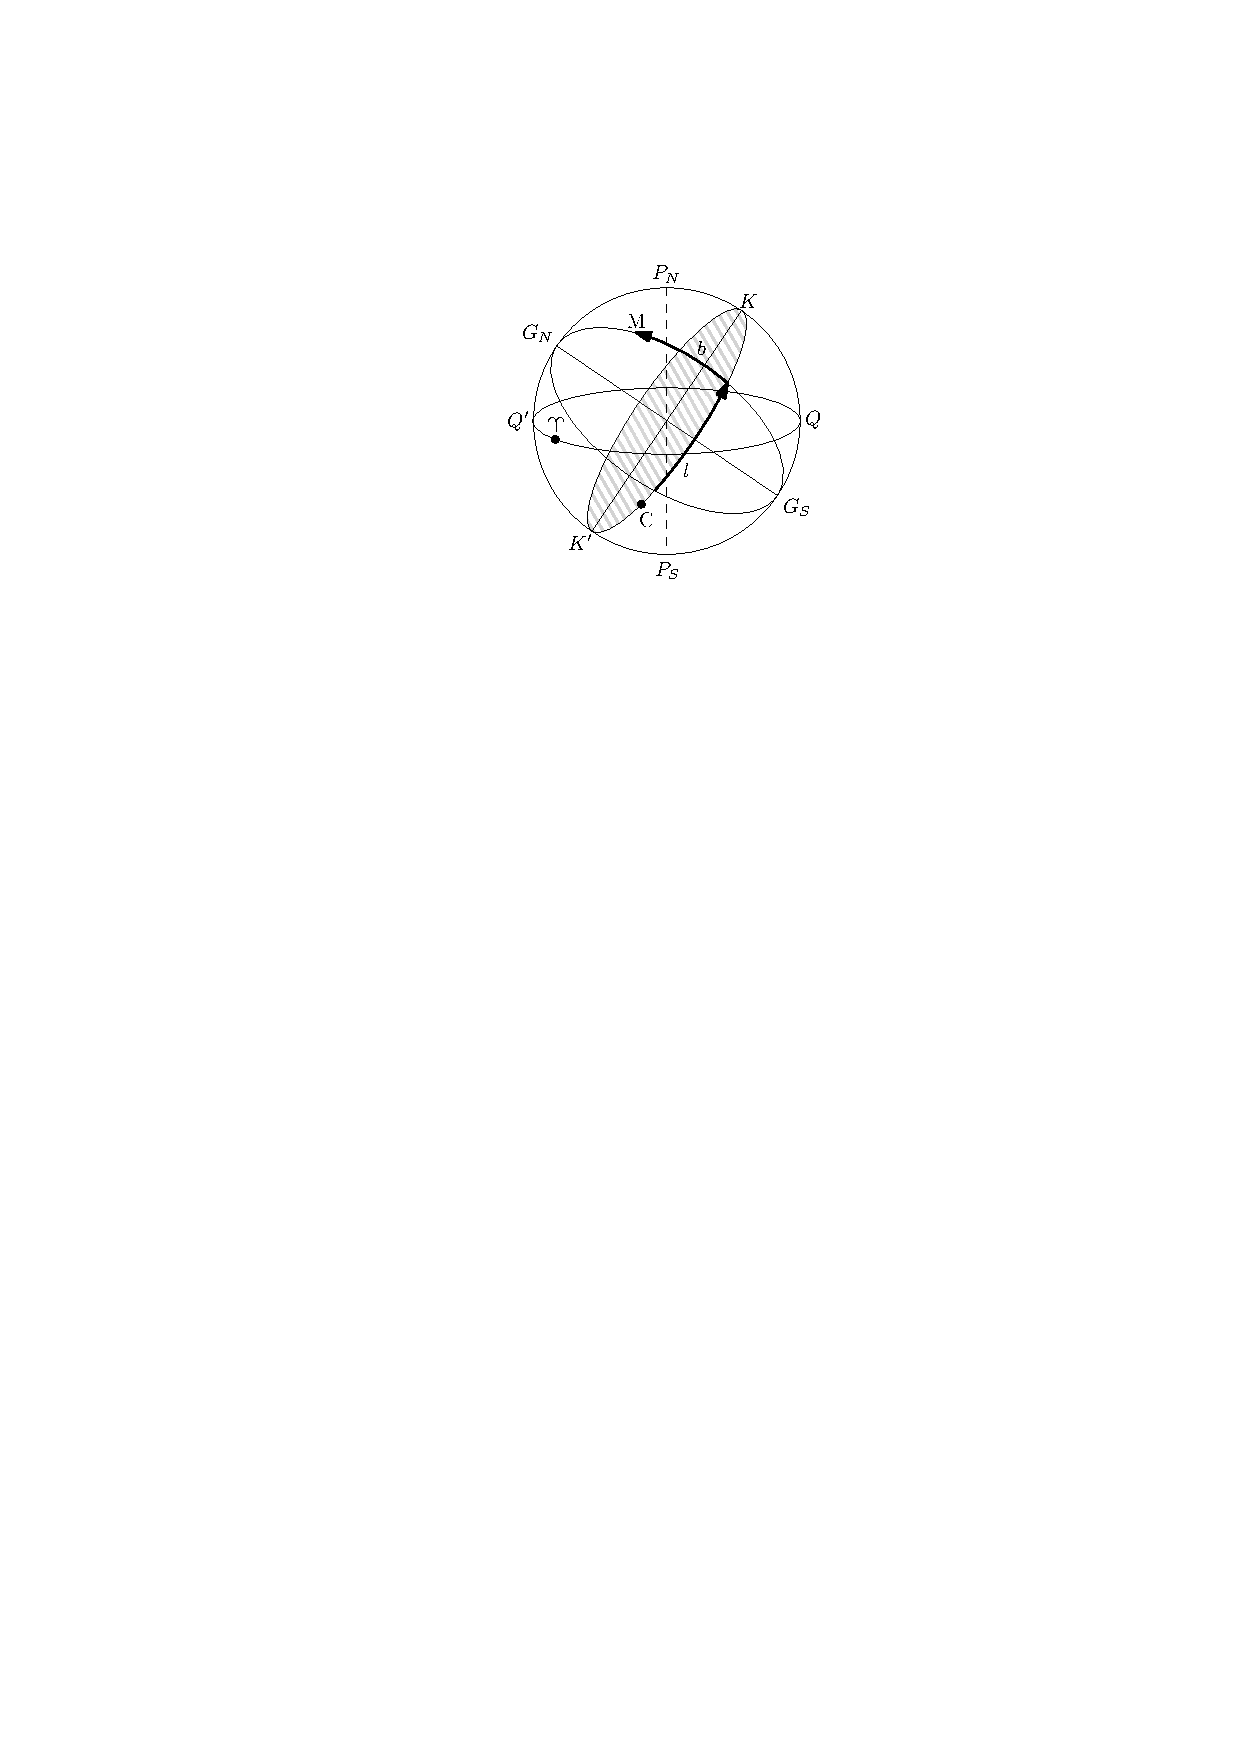
\includegraphics[width = \textwidth]{gal-coordin-sys}
		\caption{Галактическая система координат}
	\end{subcaptionblock}
	\caption{Системы координат II}
\end{figure}
\term{Эклиптическая система координат}~--- система координат, основной плоскостью которой является плоскость эклиптики $E \libra E' \aries $. Одной координатой при этом является \term{эклиптическая широта}~$\beta$~--- угловое расстояние между светилом и плоскостью эклиптики, отсчитываемое в сторону северного полюса мира, а другой~--- \term{эклиптическая долгота}~$\lambda$~--- угловое расстояние между точкой весеннего равноденствия и кругом эклиптической широты светила. Полюса эклиптики $E_N$ и $E_S$ имеют координаты ($18^h$,~$90^\circ - \varepsilon$) и ($6^h$,~$-90^\circ + \varepsilon$).

\term{Галактическая система координат}~--- система координат, основной плоскостью которой является плоскость нашей галактики, которая наклонена к плоскости небесного экватора под углом $62.6^\circ$. Одной координатой при этом является \term{галактическая широта}~$b$~--- угол между плоскостью галактического экватора и направлением на светило, а другой~--- \term{галактическая долгота}~$l$~--- угол между направлением на точку начала отсчёта $C$ и плоскостью круга галактической широты светила. Точка $C$ является направлением на центр галактики и имеет координаты: $\alpha=17^h\,45.6^m$, $\delta=-28^{\circ}\,56.2'$. $C K K'$~--- плоскость галактического экватора; $G_N$, $G_S$~--- северный и южный полюса галактики соответственно.
